\documentclass[12pt,oneside]{exam}

% This package simply sets the margins to be 1 inch.
\usepackage[margin=1in]{geometry}

% These packages include nice commands from AMS-LaTeX
\usepackage{amssymb,amsmath,amsthm,amsfonts,latexsym,verbatim,xspace,setspace, graphicx}
\usepackage{subfigure}

% Make the space between lines slightly more
% generous than normal single spacing, but compensate
% so that the spacing between rows of matrices still
% looks normal.  Note that 1.1=1/.9090909...
\renewcommand{\baselinestretch}{1.1}
\renewcommand{\arraystretch}{.91}

% Define an environment for exercises.
\newenvironment{exercise}[1]{\vspace{.1in}\noindent\textbf{Exercise #1 \hspace{.05em}}}{}
\newenvironment{newsolution}{\vspace{.1in}\noindent\textbf{Solution \hspace{.05em}}}{}

% define shortcut commands for commonly used symbols
\newcommand{\R}{\mathbb{R}}
\newcommand{\C}{\mathbb{C}}
\newcommand{\Z}{\mathbb{Z}}
\newcommand{\Q}{\mathbb{Q}}
\newcommand{\N}{\mathbb{N}}
\newcommand{\calP}{\mathcal{P}}

\DeclareMathOperator{\vsspan}{span}

\title{Math 203 - Summer II 2018: Solutions to homework 2}

%%%%%%%%%%%%%%%%%%%%%%%%%%%%%%%%%%%%%%%%%%

\begin{document}

\begin{flushright}
\sc MAT 203 - Lecture 1\\
July 25, 2018.
\end{flushright}
\bigskip

\begin{center}
\textsf{Homework 2: solutions to selected problems} 
\end{center}

\begin{exercise}{1}
Sketch the following plane curves:

\begin{parts}
\part $r(t) = (t,t^2)$.
\part $r(t)=(\cos(t), \sin(t))$.
\part $r(t)=(t^3-4t, t^2-4)$. 
\part $r(t)=(t^3,t^2)$. 
\part $r(t)=\left(\frac{3t}{1+t^3}, \frac{3t^2}{1+t^3}\right)$.
\end{parts}
\end{exercise}

\begin{newsolution}
\begin{itemize}
\item[(a)] The relationship $y=x^2$ characterizes the trace of this curve as a parabola. 
\item[(b)] The relationship $x^2+y^2 = 1$ characterizes the trace of this curve as a circle centered at the origin, with radius 1. 
\item[(c)] The relationship between the coordinates is that  $x$ and $y$ are related by multiplication by $t$, that is $t=\frac{x}{y}$ (as long as $y \neq 0$) The coordinate $y$ can be expressed by $y=t^2-4$. Thus, the parametric equations become
\begin{align*}
y & =\left(\frac{x}{y}\right)^2 -4\\
y^3 & = x^2 -4y^2.
\end{align*}
The last equation makes sense when $y=0$. You should check that the only valuee of $t$ that makes the $y$ coordinate equal to $0$ in the parametric equations are $t=-2,t=2$, whose corresponding points are $r(-2)=(0,0)$, $r(2)=(0,0)$, the same as the output of the non-parametric equations when $y=0$. A plot of the curve defined by this equation is represented below.
\begin{center}
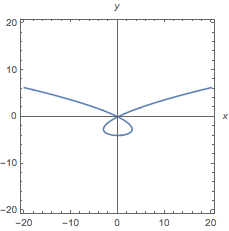
\includegraphics{hw2_plot1c.png}
\end{center}
\item[(d)] The coordinates satisfy the relation $y^3=x^2$. One can view this as the graph of the function $y(x)=x^{\frac{2}{3}}$. A plot of this graph is represented below (notice the unusual position of the axes). 
\begin{center}
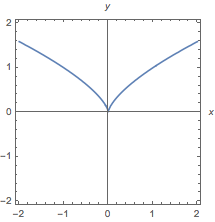
\includegraphics{hw2_plot1d.png}
\end{center}
\item[(e)] To find a relation between the coordinates that does not involve $t$ will require a bit more work than part (c), but can be done in a similar fashion. Notice that $t=\frac{y}{x}$ (as long as $x\neq 0$) this time, thus
\begin{align*}
x & = \frac{3\frac{y}{x}}{1+\left( \frac{y}{x}\right)^3}\\
x & = \frac{3y(x^3)}{x(x^3+y^3)}\\
x & = \frac{3x^2y}{x^3+y^3}
\end{align*}
Thus the parametric equations are equivalent to 
\begin{equation*}
x^3+y^3-3xy=0,
\end{equation*}
an equation which makes sense (and produces the correct output) when $x=0$. A plot of the curve defined by this equation is represented below. 
\begin{center}
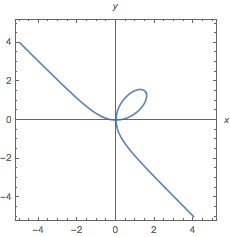
\includegraphics{hw2_plot1e.png}
\end{center}
\end{itemize} 
\end{newsolution}

\begin{exercise}{2} 
For each of the plane curves below, find the parametric equation of their tangent lines at the points indicated. 
\begin{parts}
\part $r(t)=(t,t^3)$ at the point $(2,8)$.
\part $r(t)=(\cos(t),\sin(t))$ at the point $\left(\frac{\sqrt{2}}{2}, \frac{\sqrt{2}}{2}\right)$. 
\end{parts}
\end{exercise}

\begin{newsolution}
\begin{itemize}
\item[(a)] The tangent vector to the curve at $t$ is given by $(r'(t)=(1,3t^2)$. At the point $(2,8)$, corresponding to $t=2$, this tangent vector becomes $r'(2)=(1,12)$.  The tangent line at the point $(2,8)$ can thus be described by the parametric equation
\begin{equation*}
P(s)=(2+s, 8+12s)
\end{equation*}
\item[(b)] Similar to part (a). 
\end{itemize}
\end{newsolution}

\begin{exercise}{3}
Consider the curves $r(t)=(t,t,t^2)$ and $s(t)=\left(\frac{1}{t},\frac{1}{t},0\right)$, defined for $t \neq 0$. 
\begin{parts}
\part Does the curve $r$ have a limit as $t$ goes to $0$? If so, what is the limit?
\part Does the curve $s$ have a limit as $t$ goes to $0$? If so, what is the limit?
\part Compute the dot product of the curves, $r(t) \cdot s(t)$, for $t \neq 0$. 
\part Does the scalar function obtained in part $(c)$ have a limit as $t$ goes to $0$? If so, what is this limit?
\end{parts}
\end{exercise}

\begin{newsolution}
\begin{itemize}
\item[(a)] The curve $r(t)$ tends to $(0,0,0)$ as $t \to 0$. 
\item[(b)] The curve $s(t)$ does not have a limit as $ t \to 0$, as the limits of its $x$ and $y$ coordinates are undefined. 
\item[(c)] The dot product of the curves is equal to $2$, for all $t \neq 0$. 
\item[(d)] The limit of the dot product as $t$ approaches $0$ is equal to 2. 
\end{itemize}
\end{newsolution}

\begin{exercise}{4}
An object moves in the plane according to a trajectory described by a smooth curve $r(t)$. Assume that:
\begin{enumerate}
\item the curve never passes through the origin, i.e., $r(t) \neq 0$; 
\item the velocity vector is never zero, $r'(t) \neq 0$;
\item  at time $t=0$, the curve is at its closest point to the origin.
\end{enumerate}

Explain why the position and velocity vectors $r(0)$ and $r'(0)$ are perpendicular. 
\end{exercise}

\begin{newsolution}
The distane between the object and the origin at time $t$ is given  by the magnitude of its position vector, $||r(t)||^2$. Minimizing this function and its square are equivalent problems, so we are going to study the latter in order to reduce the computations. 

The square of the lentgh of a vector can be computed in terms of the dot product, $||r(t)||^2=r(t) \cdot r(t)$. Since this scalar function has a minimum at $t=0$ , its derivative at $t=0$ is equal to $0$. By the product rule for the dot product, this implies that 
\begin{align*}
\frac{d(||r(t)||^2)}{dt} (0) & = \frac{d[r(t)\cdot r(t)]}{dt}(0) \\
0 & = 2r(0)\cdot r'(0), 
\end{align*}
hence $r(0) \cdot r'(0) = 0$, that is, position and velocity vectors are perpendicular at $t=0$. 
\end{newsolution}

\begin{exercise}{5}
Let $r(t)$ denote a spatial curve, and $r'(t)$, $r''(t)$ its first and second derivatives, respectively. Assume that $r''(t) \neq 0$. If the position $r(t)$ and acceleration $r''(t)$ are colinear, for all times, what can you say about the cross product $r(t) \times r'(t)$? 
\end{exercise}

\begin{newsolution}
If $r$ and $r''$ are aligned for all $t$, then $r(t) \times r''(t) = 0$, for all $t$. From the product formula for the cross product, 
\begin{align*}
\frac{d [r(t) \times r'(t)]}{dt} & = r'(t) \times r'(t) + r(t) \times r''(t) \\
 & =  r(t) \times r''(t)\\
 & = 0, 
\end{align*}
hence the cross product $r(t)\times r'(t)$ is constant.
\end{newsolution}

\begin{exercise}{6}
As we saw in class, the Fundamental Theorem of Calculus for Curves can be used to compute the displacement vector, 
\begin{equation*}
\int_{a}^{b} r'(t) dt = r(b)-r(a).
\end{equation*}
Use this to describe the trajectory described by a curve with velocity vector 
\begin{equation*}
r'(t)=\frac{1}{1+t^2} i + tj + e^tk, 
\end{equation*}
and which satisfies $r(0)=(1,0,-1)$. 
\end{exercise}

\begin{newsolution}
The trajectory is described by 
\begin{align*}
r(t) & = r(0) + \int_{0}^{t} r'(s) ds \\
& = i -k  + \left( \int_{0}^{t} \frac{1}{1+s^2} ds \right) i + \left( \int_{0}^{t} s ds \right)j + \left(\int_{0}^{t} e^s ds \right)k\\
& = (\arctan(t)+1) i + \frac{t^2}{2}j + {e^t}k
\end{align*}
\end{newsolution}


\begin{exercise}{7}
Find two vector functions $r(t)$ and $s(t)$ for which 
\begin{equation*}
\int[ r(t) \times s(t)] dt  \neq \left(\int r(t) dt \right) \times \left( \int s(t) dt \right)
\end{equation*}
\end{exercise}

\begin{newsolution}
There are infinitely many right answers to this problem. One of them is $r(t)=ti$, $s(t)=tj$, as you can easily verify by yourself. 
\end{newsolution}

\begin{exercise}{8}
Consider the function 
\begin{equation*}
f(x,y)=\frac{x^2y}{x^4+y^2},
\end{equation*}
defined for all points $(x,y)$ in the plane except the origin $(0,0)$. This exercise will study the behavior of this function near the origin. 

\begin{parts}
\part Compute the directed limits of this function along the lines $y=kx$, in terms of the parameter $k$. 
\part Compute the limit of this function along the parabola $y=x^2$.
\end{parts}

The results of parts $a$ and $b$ should be different. This is to show you that unlike what you studied in single-variable Calculus and what we observed for vector-valued, single-variable functions, the existence and coincidence of directed limits no longer imply the existence of the limit of the function. This marks a sharp contrast between single-variable functions and multivariable functions.
\end{exercise}

\begin{newsolution}
\begin{itemize}
\item[(a)] Replacing $y$ by $kx$ and computing the resulting limit with L'H\^opital's rule yields limit $0$, regardless of $k$. 
\item[(b)] This time replacing $y$ by $x^2$ and computing the resulting limit yields the result $\frac{1}{2}$. 
\end{itemize}
\end{newsolution}

\begin{exercise}{9}
This exercise is about the following function: 
\begin{equation*}
f(x,y) = 
\left\{
\begin{array}{rl}
\frac{y}{x}-y & \mbox{ if} \ 0 \leq y < x \leq 1 \\
\frac{x}{y}-x & \mbox{ if} \ 0 \leq x < y \leq 1 \\
1-x & \mbox{if} \ 0 <x = y < 1 \\
0 & \mbox{ elsewhere}.
\end{array}
\right.
\end{equation*}

\begin{parts}
\part Sketch the graph of this function on the square $[0,1] \times [0,1]$. 
\part What is the value of this function along the boundary of the square?
\part If the value of $x$ is kept constant, is $f$ a continuous function of $y$?
\part If the value of $y$ is kept constant, is $f$ a continuous function of $x$?
\part Compute the directed limit of the function as $(x,y)$ approaches the origin along the line $y=x$. 
\part Compare your answer of part $(e)$ with the value of the function at $(0,0)$ which you obtained in part $(b)$. Is this function continuous at $(0,0)$?
\end{parts}
\end{exercise}

\begin{newsolution}
\begin{itemize}
\item[(a)] Below are two plots of the function (notice the slightly unusual position of the axes). The region outside the square $[0,1] \times [0,1]$ was excluded from view, as it is not relevant to the problem at hand. 

\begin{figure}
\hfill
\subfigure{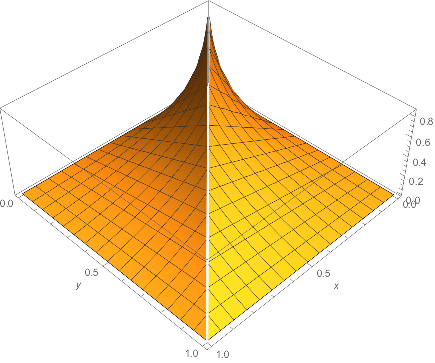
\includegraphics[width=5cm]{hw2_plot9.png}}
\hfill
\subfigure{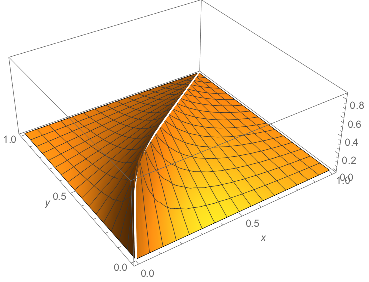
\includegraphics[width=5cm]{hw2_plot9alternative.png}}
\hfill
\end{figure}

\item[(b)] The value of the function on the boundary of the square is $0$, as it can easily be verified by checking the equations defining the function.  
\item[(c)] The function is continuous relative to the variable $y$. To verify this, notice that the pieces defining the function are the same when $y=x$, the only point at which a discontinuity could appear within the square. Outside the square, the value of the function is $0$, the same as the value on the boundary, thus there is no discontinuity there either. 
\item[(d)] Analogous to part (c). 
\item[(e)] The value of the function along the line segment $y=x$, $0< x< 1$, is given by $1-x$. The directed limit as $x$ approaches $0$ from the positive side is equal to $1$. Meanwhile, if $x$ is negative, then the value of the function is zero (since the corresponding point $(x,y)$ is outside of the square), so the  directed limit as $x$ approaches $0$ from the left is $0$. It follows that the function does not have a limit at $0$ along the line $y=x$. 
\item[(f)] The value of the function at $(0,0)$ is $0$, in contrast with the fact that the limit of the function as $(x,y)$ approaches zero does not exist. This is an example of a function which is separately continuous with respect to each variable, but not continuous in the multivariable sense. 
\end{itemize}

\end{newsolution}

\begin{exercise}{10}
Compute \textbf{all} the partial derivatives of the function $f(x,y,z)=ye^x+x\ln(z^2+1)$ up to order two. 
\end{exercise}

\begin{newsolution}
This can be done by sucessively computing single-variable derivatives. Your answers should be:
\begin{align*}
\frac{\partial f}{\partial x} & = ye^x + \ln(z^2+1) \\
\frac{\partial f}{\partial y} & = e^x\\
\frac{\partial f}{\partial z} & = \frac{2xz}{z^2+1} \\
\frac{\partial^2 f}{\partial x^2} & = ye^x \\
\frac{\partial^2 f}{\partial y^2} & = 0 \\
\frac{\partial^2 f}{\partial z^2} & = \frac{2x - 4xz^2}{(z^2+1)^2}\\
\frac{\partial^2 f}{\partial x \partial y} & = e^x \\
\frac{\partial^2 f}{\partial x \partial z} & = \frac{2z}{z^2+1}\\
\frac{\partial^2 f}{\partial y \partial z} & = 0.
\end{align*}
\end{newsolution}

\begin{exercise}{11}
Verify that the functions given satisfy the corresponding equations. 
\begin{parts}
\part The function $f(t,x)=\sin(x-t)$ satisfies \textit{the wave equation}
\begin{equation*}
\frac{\partial^2 f}{\partial t^2} = \frac{\partial^2 f}{\partial x^2}.
\end{equation*}
\part The function $f(t,x)=e^{-t}\cos(x)$ satisfies \textit{the heat equation}
\begin{equation*}
\frac{\partial f}{\partial t} = \frac{\partial^2 f}{\partial x^2}
\end{equation*}
\part The function $f(x,y)=e^x\sin(y)$ satisfies \textit{Laplace's equation}
\begin{equation*}
\frac{\partial^2 f}{\partial x^2} + \frac{\partial^2 f}{\partial y^2} = 0. 
\end{equation*}
\end{parts}
\end{exercise}

\begin{newsolution}
Simple computation.
\end{newsolution}
\end{document}


